\section{Resistencias equivalentes}
En los cálculos de resistencias equivalentes (en circuitos eléctricos, transferencia de calor o sistemas hidráulicos como se dará cuenta en algunos años más), existen dos posibles configuraciones:
\begin{figure}[h]
    \centering
    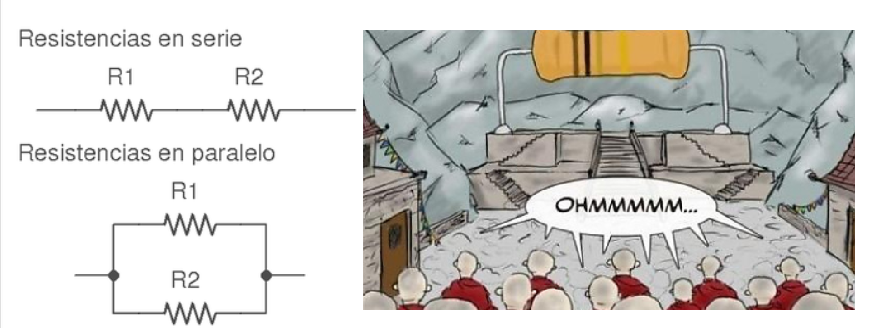
\includegraphics[scale=0.7]{Guia/resistencias.png}
    \caption{Distintas configuraciones y un chisterete}
\end{figure}
\begin{enumerate}
    \item \textbf{Serie:} Cuando en el mismo cable hay varias resistencias, el valor de la resistencia equivalente es la suma de todas las resistencias.
    \begin{equation}
        R_{eq}=R_1+R_2+...+R_n=\sum_{i=1}^n R_i
    \end{equation}
    \item \textbf{Paralelo:} Cuando las resistencias comparten dos nodos (o uniones de cables). El recíproco de la resistencia equivalente es igual a la suma de todos los recíprocos de las resistencias individuales
    \begin{equation}
        \frac{1}{R_{eq}}=\frac{1}{R_1}+\frac{1}{R_2}+...+\frac{1}{R_n}=\sum_{i=1}^n \frac{1}{R_i}
    \end{equation}
\end{enumerate}
Cree un programa que pida al usuario el tipo de configuración (serie o paralelo), la cantidad de resistencias a ingresar y luego imprima por pantalla el valor de la resistencia equivalente. Note que, en el caso de ser una configuración en paralelo, se debe elevar a -1 la suma total. 
\begin{lstlisting}[style=consola]
Ingrese configuracion (serie/paralelo): [*serie*]
Ingrese cantidad de resistencias: [*3*]
Ingrese magnitud de la resistencia 1: [*4*]
Ingrese magnitud de la resistencia 2: [*5*]
Ingrese magnitud de la resistencia 3: [*6*]
Req= 15.0
\end{lstlisting}

\begin{lstlisting}[style=consola]
Ingrese configuracion (serie/paralelo): [*paralelo*]
Ingrese cantidad de resistencias: [*2*]
Ingrese magnitud de la resistencia 1: [*2*]
Ingrese magnitud de la resistencia 2: [*2*]
Req= 1.0
\end{lstlisting}
\textbf{Hint:} Para tener un contador en el mensaje de ingreso de datos use lo siguiente
\begin{lstlisting}[style=consola]
contador=1
while condicion:
    dato=input('Ingrese dato '+str(contador)+': ')
    contador+=1
\end{lstlisting}